\chapter{Open Problems and Outlook}
\label{ch:open-problems}

\begin{chapterlead}
Non-Hermitian photonics is a young and rapidly developing field. Many
fundamental questions remain open, and new experimental platforms
continue to reveal unexpected phenomena. This final chapter surveys the
frontier as a set of tensions that drive the field forward. Each section identifies a
concrete gap between the theoretical framework of this book and the
physics that lies beyond it, explains why the gap matters, and points
toward the ideas that may close it.
\end{chapterlead}

\begin{figure}[t]
 \centering
 
\includegraphics[width=0.82\linewidth]{fig_f19_frontier_landscape.pdf}
 \caption{Seven coupled frontiers of Maxwell-first non-Hermitian
 photonics. Solid lines connect each frontier to the central Maxwell
 operator framework developed in this book; dashed lines indicate
 cross-frontier couplings where progress on one problem constrains or
 enables another. The frontiers are: nonlinear exceptional points
 (EPs), quantum noise limits, Floquet-driven media, three-dimensional
 exceptional geometry, inverse design via quasinormal modes (QNMs),
 rigorous spectral theory, and topological classification beyond
 two dimensions. Each is discussed in a section of this chapter.}
 \label{fig:frontier-landscape}
\end{figure}

%% ================================================================
\section{Nonlinear non-Hermitian photonics}
\label{sec:nonlinear-nh}

\subsection{Why linearity is not enough}
\label{ssec:nonlinear-why}

The entire theoretical framework of this book assumes linear media: the
permittivity $\epsr$ is independent of the field amplitude, and the
Maxwell operator is a fixed linear map. This assumption breaks down in
two physically important regimes:
\begin{enumerate}
 \item \textbf{Above the lasing threshold.} Once gain exceeds loss in
 a cavity mode, the field amplitude grows exponentially until gain
 saturation---a nonlinear effect---clamps it. The steady-state
 amplitude is set by the balance between saturated gain and loss,
 not by the linear eigenproblem.
 \item \textbf{Strongly driven systems.} High-intensity light in a
 Kerr medium modifies the refractive index as
 $n_{\mathrm{eff}} = n_0 + n_2\,|E|^2$, creating an
 intensity-dependent effective Hamiltonian. In a non-Hermitian system,
 the Kerr shift can move the system toward or away from an exceptional
 point, coupling the EP physics to the field dynamics.
\end{enumerate}

\subsection{Gain saturation and the fate of exceptional points}
\label{ssec:gain-saturation-open}

Gain saturation introduces a nonlinear self-consistency problem: the
effective Hamiltonian depends on the field amplitudes, which in turn
depend on the Hamiltonian. Near an EP, the consequences are subtle.
Zheng and Chong showed that in a coupled-cavity laser system, noise
fluctuations shift the operating point away from the EP, effectively
reducing the EP order and preventing the system from exploiting the full
$\epsilon^{1/n}$ responsivity~\cite{zheng2024noise}. Moreover, the
linearized Bogoliubov--de~Gennes (BdG) Hamiltonian governing small fluctuations
around the nonlinear steady state has its \emph{own} EP structure, which
can produce noise divergences \emph{stronger} than the simple Petermann
estimate from the linear system.

This result challenges the premise that operating a sensor near a linear
EP automatically confers a metrological advantage. A full theory of
nonlinear EP sensing must
treat the noise, the nonlinearity, and the EP on an equal footing,
rather than analyzing the linear EP first and adding noise afterward.

\subsection{Nonlinear topology}
\label{ssec:nonlinear-topology}

Can topological invariants survive in a nonlinear system? For Kerr-type
nonlinearity, Xia et al.\ demonstrated experimentally that local
intensity-dependent refractive index changes can tune the global $\PT$
symmetry of a waveguide lattice, restoring or destroying non-Hermitian
topological states~\cite{xia2021nonlinear}. This suggests that
nonlinearity does not simply destroy topology: in suitable driven
systems it can create an intensity-dependent topological phase
diagram~\cite{zhen2023nonlinear,xia2021nonlinear,szameit2020nonlinearity,leykam2016edge,li2022topological,kartashov2024solitons,tang2022vector}.

A systematic theory of nonlinear non-Hermitian topology~\cite{rechtsman2013photonic,kim2020recent,maczewsky2017observation,kitagawa2010topological,rudner2013anomalous,nathan2017anomalous,guglielmon2017photonic,farrell2016edge} is still
missing. The obstacles include:
\begin{itemize}
 \item Topological invariants are defined for linear eigenproblems;
 extending them to nonlinear fixed-point problems requires new
 mathematical tools.
 \item The skin effect, which depends on the spectral winding of the
 \emph{linear} Hamiltonian, may be modified or destroyed by
 nonlinear mode coupling.
 \item Solitons in $\PT$-symmetric systems form continuous families
 rather than the isolated amplitude values found in generic
 dissipative systems~\cite{wimmer2015observation,alexeeva2012optical,mukherjee2021observation,johansson2025floquet,shen2023floquet,chen2025nonlinear};
 the stability and topological classification of these families remain
 open problems.
\end{itemize}

\paragraph{Open problem: nonlinear EP laser dynamics.}
Consider a pair of coupled ring resonators with Kerr nonlinearity,
modelled by
\begin{equation}
 i\frac{\dd}{\dd t}
 \begin{pmatrix} a_1 \\ a_2 \end{pmatrix}
 =
 \begin{pmatrix}
 \omega_0 + g(|a_1|^2) + i\gamma_1 & \kappa \\
 \kappa & \omega_0 + g(|a_2|^2) - i\gamma_2
 \end{pmatrix}
 \begin{pmatrix} a_1 \\ a_2 \end{pmatrix},
 \label{eq:nonlinear-ep-laser}
\end{equation}
where $g(I) = g_0/(1 + I/I_{\mathrm{sat}})$ models gain saturation
and $\gamma_2$ represents linear loss. At low intensity the system
approaches a linear EP when $|\gamma_1 - \gamma_2| = 2|\kappa|$. But
as $|a_1|^2$ grows, the saturated gain shifts $\gamma_1$ downward,
and the instantaneous Hamiltonian moves \emph{away} from the EP.
The resulting limit cycle oscillates between near-EP and far-from-EP
regimes, producing a characteristic ``EP breathing'' in the output
intensity. Whether this breathing mode has any robust dynamical
signature tied to the nearby degeneracy---or whether it is a generic
feature of nonlinear saddle--node bifurcations near non-Hermitian
degeneracies---is an open question that requires tools from both
dynamical systems theory and non-Hermitian spectral theory.

\paragraph{Gain saturation and the Bogoliubov--de~Gennes connection.}
The fluctuation dynamics around a nonlinear steady state are governed by
a Bogoliubov--de~Gennes (BdG) Hamiltonian that couples the signal and
idler quadratures. Zheng and Chong showed that the BdG Hamiltonian can
have its own EP structure that is \emph{different} from the EP of the
underlying nonlinear Hamiltonian~\cite{zheng2024noise}. The BdG EP can
produce noise divergences that scale with a Petermann factor computed
from the BdG eigenvectors, not from the original linearized system
alone. This ``BdG Petermann effect'' is a nonlinear extension of the
linear excess-noise mechanism. Its experimental signature---anomalous
linewidth broadening controlled by the fluctuation operator rather than
only by the instantaneous mean-field Hamiltonian---has not yet been
isolated.


%% ================================================================
\section{Quantum non-Hermitian photonics}
\label{sec:quantum-nh}

\subsection{From effective Hamiltonians to open quantum systems}
\label{ssec:quantum-effective}

The effective non-Hermitian Hamiltonian $H_{\mathrm{eff}}$ used
throughout this book is derived from the full Lindblad master equation
by conditioning on zero quantum jumps. This post-selected description
captures the \emph{conditional} dynamics of the photonic system but
discards the quantum jumps (spontaneous emission events, photon
absorption by the environment) that are essential for a complete picture
of the noise and the measurement statistics.

The quantum noise theory of EP sensors~\cite{zhang2018quantum} shows
that the discarded quantum jumps reintroduce noise channels that can
cancel the apparent EP responsivity enhancement in standard measurement
settings. A consistent quantum theory of non-Hermitian photonics must
therefore start from the full open quantum system---either the Lindblad
equation or the quantum Langevin equations with input--output
formalism---and derive the non-Hermitian effective Hamiltonian as a
limit rather than a postulate.

\subsection{Few-photon non-Hermitian physics}
\label{ssec:few-photon}

Most non-Hermitian photonic experiments operate in the classical regime
(many photons per mode). In the few-photon regime, the effective
Hamiltonian description can break down because the probability of
quantum jumps during the observation time becomes significant. The
interplay of non-Hermiticity, quantum fluctuations, and
photon-number-resolved measurement creates a rich and largely unexplored
landscape.

Specific open questions include:
\begin{enumerate}
 \item Can the non-Hermitian skin effect be observed in a quantum
 photonic simulator with single-photon resolution?
 \item Under what measurement protocol, if any, does the EP
 responsivity enhancement translate into improved precision at the
 single-photon level?
 \item Can quantum error correction or reservoir engineering be used to
 control jump-induced decoherence in non-Hermitian topological
 states~\cite{gao2024quantum,al2024topological,acn2018quantum}?
\end{enumerate}

\subsection{Entanglement and biorthogonality}
\label{ssec:entanglement}

The biorthogonal basis (Appendix~\ref{app:nonnormal}) is a mathematical
tool for expanding observables in a non-Hermitian system. Whether it has
a direct quantum information interpretation---for example, whether the
biorthogonal entanglement entropy captures physically relevant
correlations in an open photonic system---is an open and active question.


%% ================================================================
\section{Time-varying and Floquet non-Hermitian systems}
\label{sec:floquet-nh}

\subsection{Floquet engineering of non-Hermiticity}
\label{ssec:floquet-engineering}

Time-periodic (Floquet) modulation of the refractive index creates
effective non-Hermitian Hamiltonians with periodically driven gain, loss,
and coupling. The Floquet formalism maps the time-dependent problem
onto a static problem in an extended Hilbert space (the Floquet--Bloch
space), where the effective Hamiltonian can exhibit EPs, $\PT$ symmetry,
and topological phases that do not exist in any static system.

\begin{figure}[t]
 \centering
 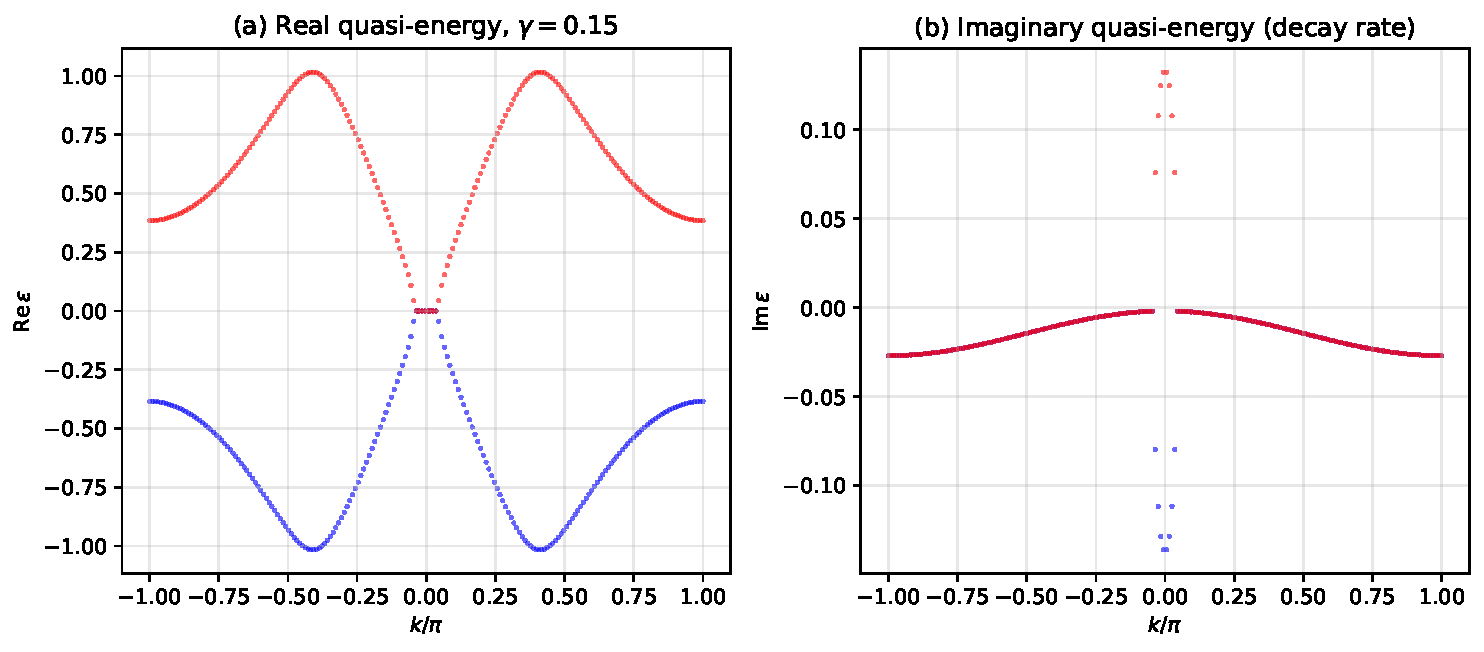
\includegraphics[width=0.85\linewidth]{figures/fig_f19_floquet_bands.pdf}
 \caption{Floquet quasi-energy bands for a periodically driven
 non-Hermitian two-band model ($\gamma = 0.15$, $V = 0.8$,
 $\Omega = 2.5$). (a)~Real part of the quasi-energy $\varepsilon(k)$,
 showing the band structure folded into the Floquet--Brillouin zone.
 (b)~Imaginary part of $\varepsilon(k)$, representing the decay rate.
 The asymmetry between the two bands reflects the non-Hermiticity.}
 \label{fig:floquet-bands}
\end{figure}

\subsection{Floquet exceptional points}
\label{ssec:floquet-ep}

A Floquet EP occurs when two Floquet quasi-energies coalesce---not
necessarily because the instantaneous Hamiltonian has an EP at any fixed
time, but because the time-ordered evolution operator over one period
has a Jordan-block structure. Floquet EPs can be created and controlled
by the modulation amplitude and frequency, providing a temporal knob for
EP physics in addition to spatial design.

\paragraph{Example: periodically modulated coupled cavities.}
Consider two coupled cavities with time-periodic detuning:
$\delta(t) = \delta_0 \cos(\Omega t)$, where $\Omega$ is the
modulation frequency. In the Floquet--Bloch representation, the
effective Hamiltonian becomes an infinite-dimensional matrix coupling
all Floquet harmonics $n\Omega$. A Floquet EP appears when the
modulation amplitude $\delta_0$ reaches a critical value at which two
Floquet quasi-energy bands touch and coalesce. Unlike a static EP, the
degeneracy is defined modulo the drive frequency and can involve
different Floquet replicas; it can therefore be tuned by varying
$\Omega$ or the modulation strength without changing the spatial
geometry. Its stability, however, still depends on the usual
codimension and symmetry constraints of the driven non-Hermitian
operator.

The physical signature is a characteristic beating pattern in the
transient response: near the Floquet EP, the temporal evolution contains
a term proportional to $t\,e^{-i\varepsilon t}$ (the Jordan-block
contribution), producing a linear-in-$t$ envelope modulating the
oscillatory response. This temporal signature is the Floquet analogue
of the spatial mode coalescence at a static EP and can be measured in
the time-domain transmission of a pulsed probe.
\begin{figure}[t]
 \centering
 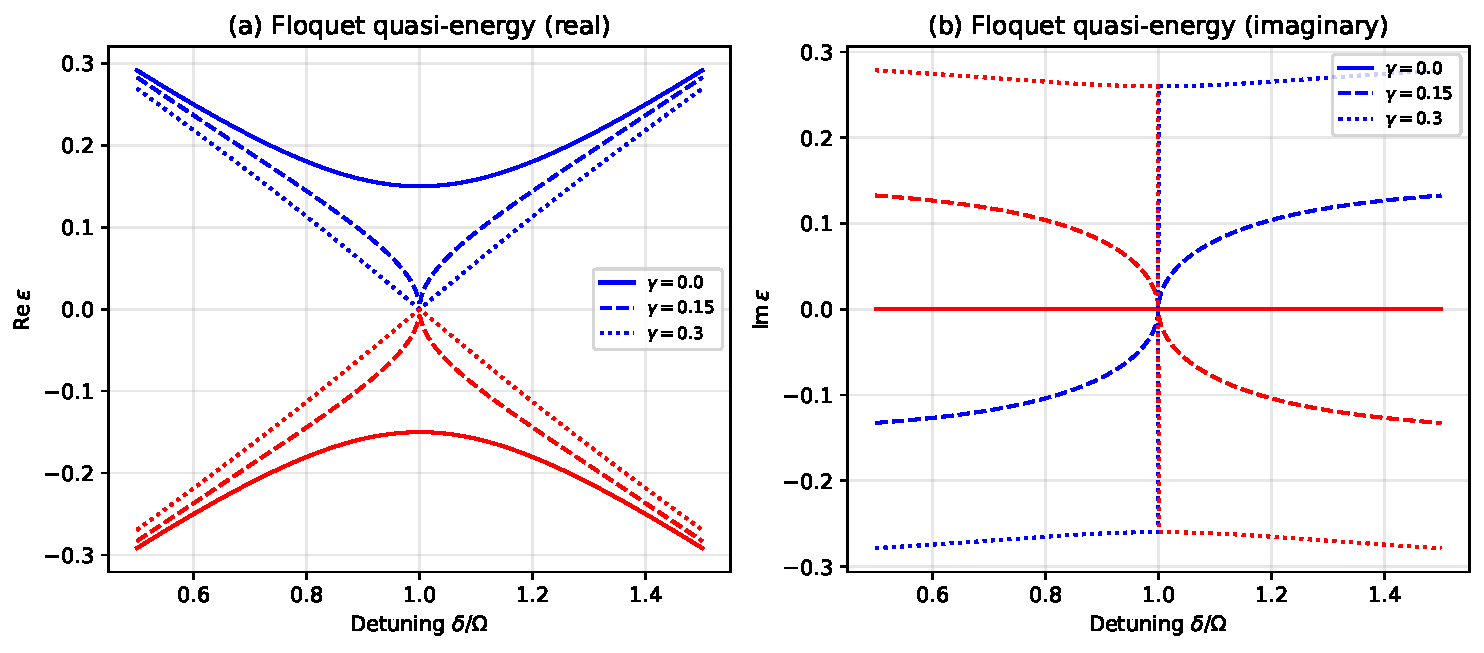
\includegraphics[width=0.85\linewidth]{figures/fig_f19_floquet_ep.pdf}
 \caption{Floquet exceptional point in a periodically driven two-mode
 model. The rotating-wave Floquet Hamiltonian develops quasi-energy
 coalescences controlled by detuning and modulation amplitude.
 (a)~Real quasi-energies show avoided crossings and coalescence as the
 non-Hermitian parameter increases. (b)~Imaginary quasi-energies reveal
 the gain--loss splitting associated with the Floquet EP. The point of
 the figure is not a new device proposal but the mechanism: a time-periodic
 Maxwell system can acquire non-Hermitian degeneracies in Floquet space
 even when no static instantaneous Hamiltonian sits at an EP.}
 \label{fig:floquet-ep}
\end{figure}


\subsection{Open problems}
\label{ssec:floquet-open}

The interplay of temporal and spatial periodicity in non-Hermitian
systems creates several open problems:
\begin{itemize}
 \item A general bulk-boundary correspondence for Floquet
 non-Hermitian systems is not yet established.
 \item The non-Hermitian skin effect in Floquet systems can depend on
 both the driving frequency and the spatial boundary conditions,
 leading to a richer phase diagram than the static case.
 \item Experimental realization of Floquet non-Hermitian photonics
 requires modulation at optical frequencies, which is technically
 demanding but may be achievable with electro-optic modulators or
 optomechanical coupling.
\end{itemize}


%% ================================================================
\section{Non-Hermitian photonics in three dimensions}
\label{sec:3d-nh}

\subsection{Exceptional lines and surfaces}
\label{ssec:3d-topology}

Three-dimensional non-Hermitian photonic crystals support topological
objects that have no lower-dimensional counterpart:
\begin{itemize}
 \item \textbf{Exceptional lines:} one-dimensional curves in the 3D
 Brillouin zone where two bands coalesce. The topology of an
 exceptional line is characterized by a topological charge
 (a $\pi$ Berry phase encircling the line) and a linking number with
 other exceptional lines.
 \item \textbf{Exceptional surfaces:} two-dimensional manifolds of
 degeneracy, which can occur when additional constraints, symmetries,
 or material parameters reduce the effective codimension.
 \item \textbf{Non-Abelian charges:} when three or more bands are
 involved, the braid group replaces the simple winding number, and
 the topological classification becomes non-Abelian.
 \item \textbf{Three-dimensional skin effect:} an extensive set of
 eigenstates can localize on boundaries of a 3D sample, with the
 localization pattern depending on spectral winding and sample geometry.
\end{itemize}

\paragraph{Exceptional lines from Maxwell symmetries.}
In a generic two-band non-Hermitian problem, the EP condition imposes
two real constraints, so in a three-dimensional control space the EP set
is generically a curve. Photonic crystals can realize such control
spaces through Bloch wave vector, material parameters, or symmetry
constraints. The Maxwell vector nature adds polarization structure:
near an exceptional line the coalescing modes may carry a half-integer
vorticity or Berry phase, but the precise relation to polarization
vortices depends on the radiation channels and symmetries of the
particular structure.

\paragraph{Knotted exceptional lines.}
Exceptional lines in 3D can form knots and links. Two exceptional
lines can have a nontrivial linking number, meaning they cannot be
separated by any continuous deformation that preserves the band gap.
This linking is a topological invariant that has no 2D or 1D analogue
and represents a genuinely new form of non-Hermitian topology. Whether
knotted exceptional lines can be realised in a photonic crystal with
practical material parameters is an open fabrication challenge.

\paragraph{3D non-Hermitian skin effect and geometry dependence.}
In three dimensions, the skin effect can become geometry-dependent: the
localization boundary is determined by the interplay of spectral winding
in different spatial directions and the sample shape. In simple
separable models a rectangular sample may exhibit corner accumulation,
whereas other boundary geometries can redistribute the same non-Bloch
decay toward edges or surfaces. The geometry dependence means that the
finite-sample OBC spectrum is not determined by the conventional Bloch
band structure alone.

\subsection{Fabrication and characterization challenges}
\label{ssec:3d-challenges}

Experimental realization of 3D non-Hermitian photonic structures requires
fabrication of three-dimensional lattices with controlled, spatially
varying gain and loss---a significantly harder problem than the 1D or 2D
case. Two-photon lithography, self-assembly, and holographic patterning
are candidate technologies, but none has yet produced a 3D non-Hermitian
photonic crystal with sufficient quality for topological measurements.

Characterization is equally challenging: the 3D bulk--boundary
correspondence predicts surface, hinge, and corner modes that require
spatially resolved measurements in all three dimensions. Near-field
scanning or tomographic reconstruction may be needed.


%% ================================================================
\section{Rigorous spectral theory of open Maxwell operators}
\label{sec:spectral-theory}

\subsection{Completeness of QNM expansions}
\label{ssec:qnm-completeness-open}

The quasinormal-mode expansion (Chapter~\ref{ch:qnm}) is widely used but
not rigorously justified in full generality. The QNMs of an open
resonator form a countable set, but their completeness---in the sense
that any compactly supported source field can be expanded in QNMs---has
been proven only for specific geometries (1D slabs, spheres). For
general 3D resonators with complex shapes and dispersive materials, the
completeness question remains open.

The difficulty is mathematical: QNM fields diverge outside the
resonator (they satisfy outgoing boundary conditions at infinity), so
the expansion converges only in a distributional or regularized sense
(e.g., inside the PML region). A rigorous theory must specify the
function space in which completeness holds and the rate of convergence
of the modal sum.

\paragraph{What a completeness proof would need.}
A satisfactory proof of QNM completeness for a general 3D open Maxwell
system would need to:
\begin{enumerate}
 \item Specify the function space $\mathcal{H}$ of source/field
 distributions (e.g., $L^2$ functions with compact support inside
 the resonator volume).
 \item Prove that the set of QNM fields
 $\{\EE_m(\rr)\}_{m=1}^{\infty}$, regularized by a PML or
 complex-coordinate transformation, is dense in $\mathcal{H}$.
 \item Provide error bounds for the truncated expansion: given $N$
 modes, how large is the remainder in terms of the quality
 factors $Q_m$ and the spectral density near the target
 frequency?
 \item Handle the branch-cut contributions from the continuous
 spectrum (radiation modes), either by including them explicitly
 or by proving that the PML discretizes them into a sequence
 of discrete poles that converges to the branch cut.
\end{enumerate}
A partial result in this direction was obtained for 1D scattering
problems using Mittag-Leffler-type meromorphic expansions of the Green
function. Such results rely on the analytic structure and growth bounds
of the particular scattering problem; extending them to 3D Maxwell
systems with dispersive media requires controlling the Green tensor at
large complex frequency and accounting for branch cuts---nontrivial
analytic estimates.

\subsection{Continuous spectrum and branch cuts}
\label{ssec:continuous-spectrum}

In addition to the discrete QNM poles, the Green tensor of an open
Maxwell system has branch-cut contributions from the continuous spectrum
(radiation modes). These contributions are responsible for the ``PML
modes'' of Chapter~\ref{ch:numerics} and are essential for completeness.
A full modal expansion must include both the discrete poles and the
branch-cut integral, with quantitative estimates for the error of
truncating the branch-cut contribution.

\subsection{Spectral singularities}
\label{ssec:spectral-singularities}

A spectral singularity is a point on the real frequency axis where the
resolvent of the Maxwell operator diverges without an associated
normalizable eigenfunction---it is neither a bound state nor a
scattering resonance, but a divergence of the scattering amplitude.
Spectral singularities have been linked to lasing and CPA in
$\PT$-symmetric systems, but their mathematical theory (existence,
genericity, stability under perturbation) is not yet complete for
the full Maxwell operator with dispersive materials.


%% ================================================================
\section{Inverse design with non-Hermitian constraints}
\label{sec:inverse-design}

Computational inverse design (topology optimization, adjoint methods)
has become central to Hermitian photonic device design. Extending these
methods to non-Hermitian targets---designing a structure that places an
EP at a specified frequency, maximizes the Petermann factor, or
realizes a specific topological phase---requires new objective functions
and sensitivity formulas.

The biorthogonal perturbation theory of Chapter~\ref{ch:qnm} provides
the adjoint sensitivities needed for gradient-based optimization, but
turning these sensitivities into robust design algorithms remains a
nontrivial numerical problem.

\begin{figure}[t]
 \centering
 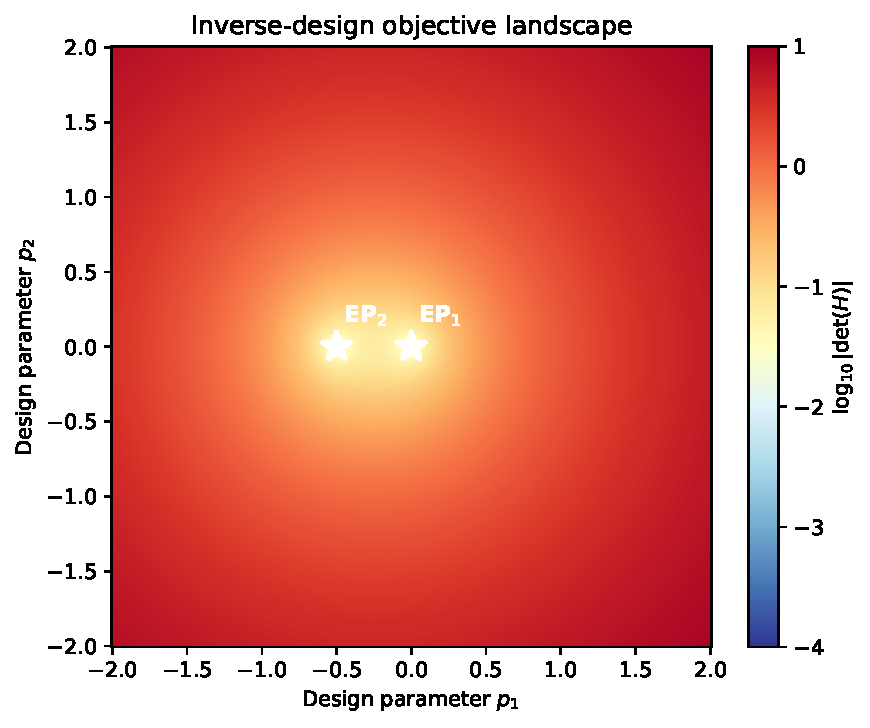
\includegraphics[width=0.6\linewidth]{figures/fig_f19_inverse_design.pdf}
 \caption{Inverse-design objective landscape $\log_{10}|\det H|$ in a
 two-parameter space. The two exceptional points (white stars) appear
 as deep minima where $\det H \to 0$. Gradient-based optimizers must
 navigate this non-convex landscape; adjoint sensitivity formulas from
 QNM perturbation theory provide the required gradients.}
 \label{fig:inverse-design}
\end{figure}

\begin{itemize}
 \item \textbf{EP targeting:} the EP is a codimension-2 degeneracy in
 parameter space; designing a structure that hits an EP at a target
 frequency requires simultaneous tuning of two real parameters.
 \item \textbf{Topological constraints:} enforcing a topological
 invariant (Chern number, winding number, BIC charge) during
 optimization requires discrete-valued objective functions, which
 are not differentiable.
 \item \textbf{Physical realizability:} optimized permittivity
 profiles must satisfy the Kramers--Kronig relations
 (Chapter~\ref{ch:loss-gain-dispersion}), and the gain/loss
 distribution must be achievable with a practical pump geometry.
\end{itemize}

\paragraph{Adjoint sensitivity for non-Hermitian objectives.}
The key technical ingredient for gradient-based inverse design is the
adjoint sensitivity: the derivative of an objective function $\mathcal{F}$
with respect to a material parameter $p$ (e.g., a pixel of $\epsr$).
For a Hermitian system, the adjoint field is the standard conjugate
field. For a non-Hermitian system, the adjoint field must be computed
from the \emph{left} eigenvector or the adjoint Green function, which
introduces the biorthogonal framework of Chapter~\ref{ch:qnm} into the
optimization loop.

For a nondispersive scalar perturbation, the leading sensitivity of a
QNM eigenfrequency $\tilde{\omega}_m$ to a local perturbation
$\delta\epsr(\rr)$ has the schematic form
\begin{equation}
 \frac{\partial\tilde{\omega}_m}{\partial\epsr(\rr)}
 = -\frac{\tilde{\omega}_m}{2}
 \frac{\tilde{\EE}_m(\rr) \cdot \tilde{\EE}_m(\rr)}
 {\langle\tilde{\EE}_m | \epsr | \tilde{\EE}_m\rangle_{\mathrm{bi}}},
 \label{eq:qnm-sensitivity}
\end{equation}
where the denominator represents the appropriate PML-regularized QNM
normalization of Chapter~\ref{ch:qnm}; dispersive, anisotropic, or
magnetic media require the corresponding generalized bilinear form.
This formula is the non-Hermitian generalisation of standard cavity
perturbation theory and provides an efficient route to gradient
computation: one adjoint solve per objective, regardless of the number
of design parameters.

\paragraph{Multi-objective design: EP + topology + noise.}
The most ambitious inverse-design target combines an EP at a specified
frequency, a topological invariant of a given value, and a noise figure
below a threshold. This is a multi-objective, mixed-integer,
Kramers--Kronig-constrained optimization problem that lies beyond
current methods. Developing efficient algorithms for this class of
problems would have immediate practical impact on the design of EP
sensors, topological lasers, and non-Hermitian metasurfaces.


%% ================================================================
\section{Energy, entropy, and thermodynamics}
\label{sec:thermodynamics}

The auxiliary-field construction of
Chapter~\ref{ch:loss-gain-dispersion} shows how to define a conserved
energy for the full field--matter system, even in the presence of
dispersion and dissipation. This construction embeds the non-Hermitian
Maxwell problem into a larger Hermitian system, where standard
thermodynamic concepts (entropy, temperature, free energy) are
well defined.

Whether this embedding can be used to define meaningful thermodynamic
quantities for the non-Hermitian photonic subsystem, and which
quantities remain subsystem-dependent bookkeeping choices, is an
intriguing open question. Specific directions
include:
\begin{itemize}
 \item Defining an entropy production rate for a non-Hermitian
 photonic mode in terms of the energy flow into the auxiliary
 (matter) degrees of freedom.
 \item Connecting the Petermann factor to a thermodynamic cost of
 maintaining a non-orthogonal mode structure.
 \item Establishing fluctuation--dissipation relations for
 non-Hermitian photonic systems that go beyond the standard
 equilibrium results.
\end{itemize}


%% ================================================================
\section{Beyond photonics}
\label{sec:beyond-photonics}

The mathematical framework developed in this book---complex eigenvalues,
biorthogonality, exceptional points, point-gap topology, the skin
effect---applies to any wave system with gain, loss, or non-reciprocity.
Active research frontiers include:

\paragraph{Acoustics and mechanics.}
Coupled acoustic resonators with active feedback and metamaterial
lattices with programmed damping provide macroscopic platforms where
non-Hermitian topology can be tested with tabletop experiments. The
slower wave speeds and larger wavelengths make spatial measurements
easier than in photonics.

\paragraph{Electronics.}
Non-Hermitian circuit lattices (topolectric circuits) with resistive
and reactive elements can realize non-Hermitian tight-binding models
with high controllability. The skin effect, point-gap topology, and
higher-order corner modes have all been observed in electronic circuits.

\paragraph{Cold atoms and condensates.}
Atomic gases with controlled loss (via resonant light or atom removal)
and effective non-Hermitian band structures provide a quantum platform
where the interplay of non-Hermiticity and interactions can be studied
in a controllable setting.

\paragraph{Condensed matter.}
Quasiparticle lifetimes in correlated electron systems generate effective
non-Hermitian self-energies. Point-gap topology and non-Hermitian
self-energy effects have been proposed as possible ingredients in
anomalous surface responses of certain topological semimetals, although
their direct relation to the skin effect in electronic materials remains
subtle.


%% ================================================================
\section{Toward a Maxwell-first synthesis}
\label{sec:maxwell-synthesis}

This monograph has consistently derived non-Hermitian phenomena from the
Maxwell equations rather than postulating them from finite-dimensional
models. Several directions remain where a Maxwell-first approach could
sharpen the understanding:

\paragraph{Topological classification of Maxwell systems.}
The 38-fold classification of non-Hermitian topological phases
(Chapter~\ref{ch:complex-bands}) was developed for tight-binding
Hamiltonians. Lifting it to the continuous Maxwell operator---with its
vector nature, gauge redundancy, and frequency-dependent material
response---is an open problem that could reveal new topological phases
unique to electromagnetism.

The vector nature is the most immediate obstacle: the Maxwell operator
acts on six-component fields $(\EE, \HH)$, not on scalar wave functions.
The polarization degree of freedom couples to the spatial structure
through the boundary conditions and the dielectric tensor, creating a
richer symmetry landscape than the scalar case. For example, a photonic
crystal with time-reversal symmetry and $C_4$ spatial symmetry can
support polarization-dependent topological phases where the TE and TM
sectors have different topological invariants---a situation that has no
analogue in electronic systems where spin--orbit coupling mixes the
spin channels.

\paragraph{Unified energy--topology--noise framework.}
The conserved energy (Chapter~\ref{ch:loss-gain-dispersion}), the
topological invariants (Chapters~\ref{ch:berry-maxwell}--\ref{ch:bbc-rebuilt}),
and the noise limits (Chapter~\ref{ch:devices}) are currently treated as
separate aspects of non-Hermitian photonics. A unified framework that
connects energy conservation, topological robustness, and noise bounds
would be a major theoretical advance---and one that can
only be formulated at the Maxwell level, where all three ingredients
coexist naturally.

A hint of such a connection comes from the Petermann factor: it appears
both as a noise amplification factor (Chapter~\ref{ch:qnm}) and as a
measure of the non-orthogonality of the eigenmodes. Near an EP, the
Petermann factor diverges, the topological charge of the EP is
non-trivial, and the energy stored in the mode becomes anomalously
large relative to the input power. Whether these three divergences are
different facets of a single geometric--thermodynamic quantity---perhaps
a non-Hermitian analogue of the Fisher information metric---is a
compelling open question.

\paragraph{A constrained optimisation perspective.}
The unification problem can be cast as a constrained optimisation over
the design space of non-Hermitian photonic structures. Let
$\mathbf{p}$ denote the design parameters (geometry, material
composition, gain--loss distribution). A device design must
simultaneously satisfy:
\begin{enumerate}
 \item \emph{Topological robustness}: the topological invariant
 $\nu(\mathbf{p})$ (Chern number, winding number, or BIC charge) must
 take a specified integer value.
 \item \emph{Noise bounds}: the Petermann factor
 $K(\mathbf{p})$ must remain below a threshold set by the
 application-level signal-to-noise requirement.
 \item \emph{Gain saturation}: the steady-state intensity
 $I_{\mathrm{ss}}(\mathbf{p})$ must lie within the linear regime
 $I_{\mathrm{ss}} < I_{\mathrm{sat}}$ for the linear non-Hermitian
 model to be valid.
 \item \emph{Fabrication robustness}: the sensitivity
 $\|\partial\nu/\partial\mathbf{p}\|$ must be small enough that
 fabrication disorder does not close the relevant gap or destroy the
 desired boundary response.
\end{enumerate}
These four constraints define a feasible region in design space. The
open question is whether this feasible region is generically nonempty:
can one simultaneously have strong topological robustness
\emph{and} low noise \emph{and} operate below saturation? The
Petermann-factor divergence at EPs
(Chapter~\ref{ch:exceptional-points}) suggests a fundamental tension
between EP-based enhancement and noise, but it is not known whether
alternative mechanisms---such as symmetry- or topology-guided BICs
(Chapter~\ref{ch:bic-topology})---can improve the tradeoff in practical
devices.

A formal optimisation objective that captures this tension is
\begin{equation}
 \min_{\mathbf{p}} \Bigl\{
 -Q_{\mathrm{topo}}(\mathbf{p})
 + \lambda_1\,K(\mathbf{p})
 + \lambda_2\,\frac{I_{\mathrm{ss}}(\mathbf{p})}{I_{\mathrm{sat}}}
 + \lambda_3\,R_{\mathrm{fab}}(\mathbf{p})
 \Bigr\},
 \label{eq:unified-objective}
\end{equation}
where $Q_{\mathrm{topo}}$ is a topological quality metric (e.g.\ the
bulk or point gap supporting the invariant), $K$ is the Petermann factor,
$I_{\mathrm{ss}}/I_{\mathrm{sat}}$ measures the proximity to gain
saturation, $R_{\mathrm{fab}}$ is a fabrication-sensitivity measure, and
$\lambda_i$ are Lagrange-like weights. Solving this optimisation
requires the adjoint sensitivity formulas of
Section~\ref{sec:inverse-design}---themselves an open problem for
non-Hermitian objectives, where the adjoint operator is not the
Hermitian conjugate but the biorthogonal partner.

\paragraph{Stable invariants for nonlinear Maxwell operators.}
The deepest mathematical question in this programme is whether
topological invariants can be defined for nonlinear, noisy Maxwell
operators. The current classification
(Chapter~\ref{ch:complex-bands}) assumes a linear Bloch Hamiltonian;
gain saturation (Chapter~\ref{ch:loss-gain-dispersion}) makes the
effective permittivity intensity-dependent, so the Hamiltonian itself
depends on the solution. Whether a meaningful topological invariant
survives in this self-consistent regime---and whether it can be computed
from a linearised operator around the steady state---is unknown.
Partial answers exist for specific models (e.g.\ the nonlinear SSH
model with Kerr coupling~\cite{hill2026exceptional}), but a general
theory for continuous Maxwell systems with dispersive, nonlinear,
and noisy materials remains an open frontier.

\paragraph{From Maxwell to field theory.}
The Maxwell operator in a periodic non-Hermitian medium is formally a
non-self-adjoint elliptic operator on a fibre bundle over the Brillouin
torus. The topological invariants of Chapters~\ref{ch:berry-maxwell}
through~\ref{ch:bbc-rebuilt} are characteristic classes of this bundle.
A field-theoretic formulation---using the language of differential
geometry and gauge theory---could clarify which invariants survive for
continuous, dispersive Maxwell operators. One possible starting point is
a non-Hermitian analogue of index theorems that relate boundary
responses to a topological index computed from the bulk Maxwell
operator.
Whether such a theorem exists for non-self-adjoint operators---and
whether it can be proven with the regularity available for Maxwell
systems with dispersive media---is a deep mathematical question at the
intersection of spectral theory, differential geometry, and photonics.

\begin{takeaway}[A field in motion]
Non-Hermitian photonics has grown quickly from a mathematical theme into
an experimental and theoretical field. Combining Maxwell's equations with
non-Hermitian spectral theory gives a disciplined way to pose its open
problems, from nonlinear topology to the thermodynamics of
non-orthogonal modes. The tools assembled here---the Maxwell eigenproblem,
the biorthogonal expansion, the GBZ, and topological charge---are starting
points for that next stage.
\end{takeaway}
